\documentclass[11pt,a4paper]{article}
\usepackage[utf8]{inputenc}
\usepackage[french]{babel}
\usepackage[T1]{fontenc}
\usepackage{amsmath}
\usepackage{amsfonts}
\usepackage{amssymb}
\usepackage{makeidx}
\usepackage{graphicx}

\usepackage{tcolorbox}

\usepackage{lmodern}

\usepackage[left=2cm,right=2cm,top=2cm,bottom=2cm]{geometry}
\author{AMONA Birewa Audrey}
\title{ Tp 06 Sécurité et site administration }
\begin{document}
\maketitle
\tableofcontents
\begin{abstract}
Ce TP contient 3 parties indépendantes. D’abord nous nous pencherons sur l’authentification. En-
suite nous explorerons les problèmes de sécurité : CSRF, HTTPS, clé de chiffrement et détournement
de clic. Enfin nous verrons comment customiser le site d’administration.
\end{abstract}
\section{Authentification}
\begin{enumerate}
\item Dans le Tp précédent, nous avions spécifié les différentes fonctionnalités en fonction des utilisateurs du système:
\begin{center}
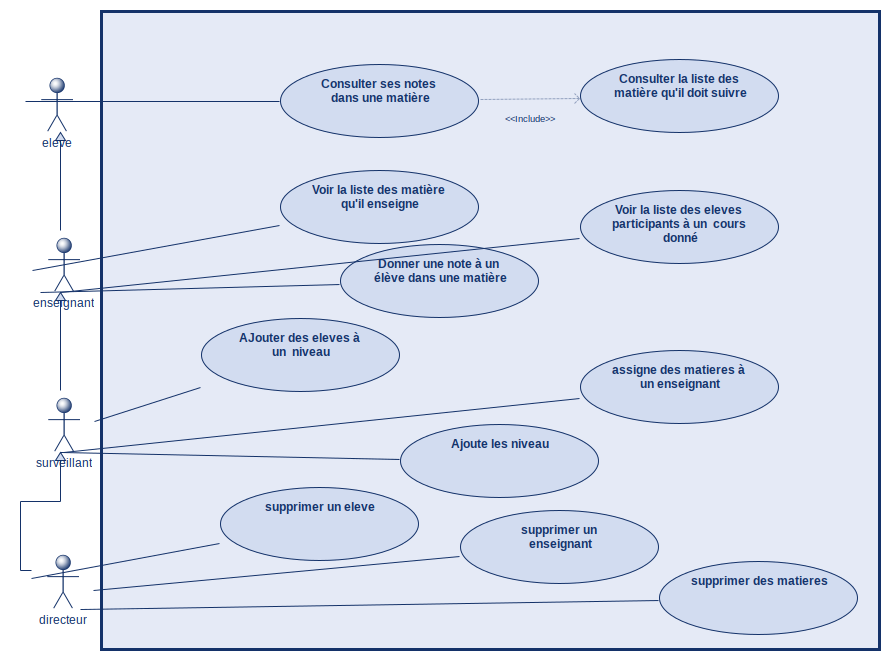
\includegraphics[scale=0.4]{images/cas.png}
\end{center}
Il étais convenu que seul les enseignant, les surveillants ou encore le directeur peuvent avoir accès au formulaire d'ajout de note.
\item Dans le site administration, nous remarquons qu'il y'a deux modèles de plus \textbf{ Users} et \textbf{Groups}, que nous n'avons pas ajouté nous même. Le modèle \textbf{Users} possède les attributs suivant: username, lastname, firstname, email adress, staff, status. Ilpossède un enregistrement qui a pour username le nom de notre superutilisateur créé.

\item Nous allons créer des groupes avec les différents roles du diagramme de cas d'utilisation précédent.
\begin{center}
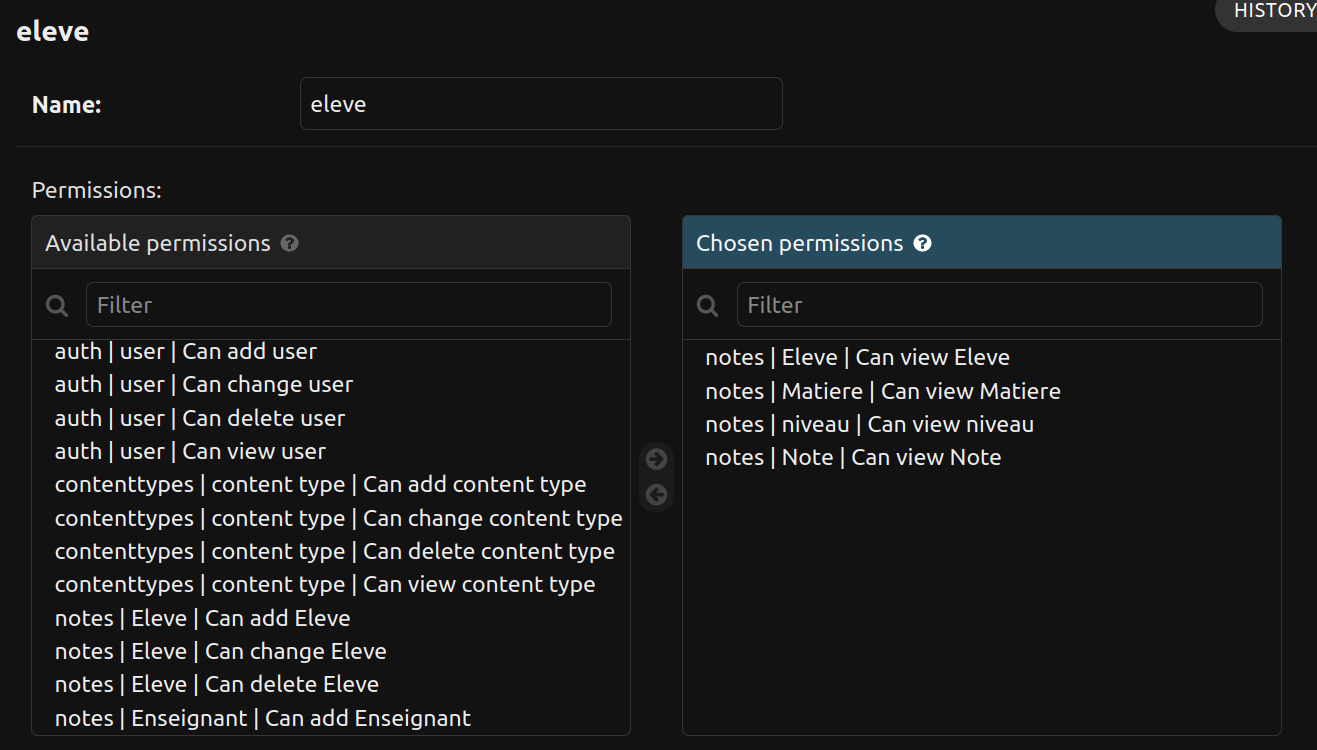
\includegraphics[scale=0.3]{images/1.png}
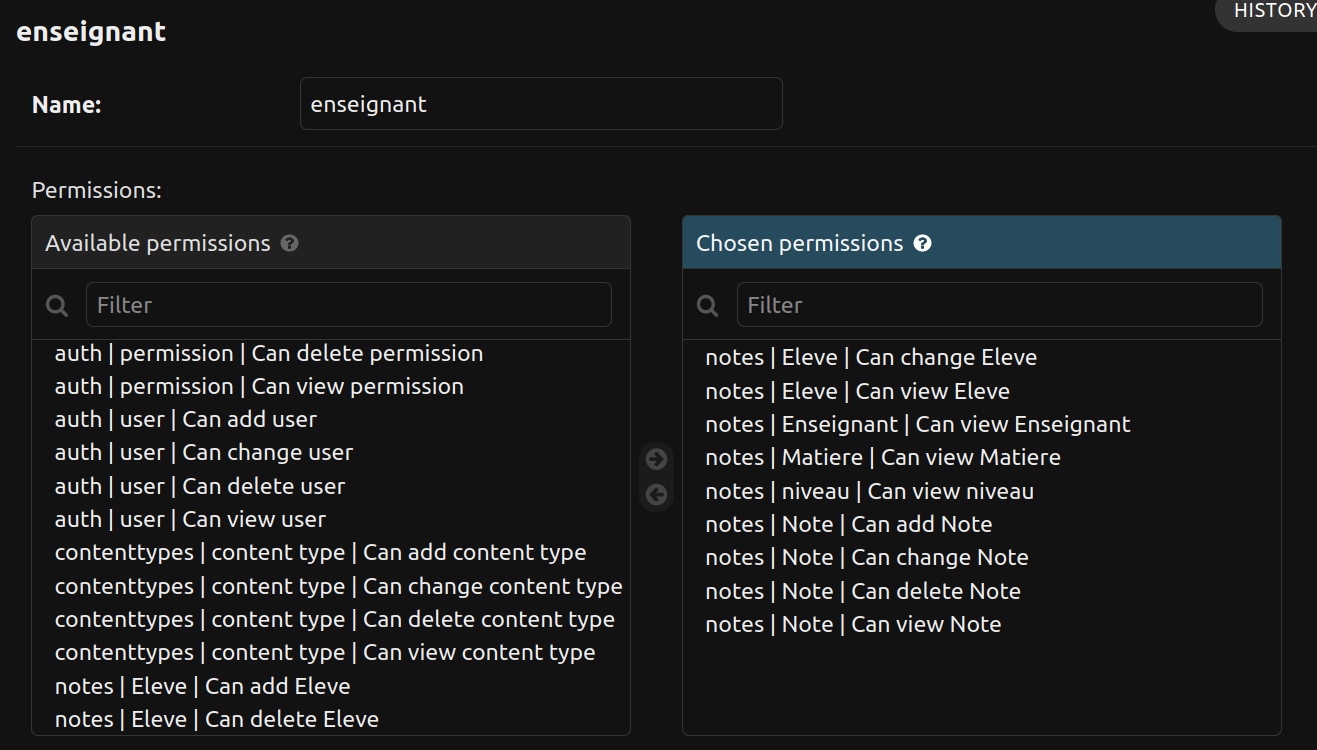
\includegraphics[scale=0.3]{images/2.png}
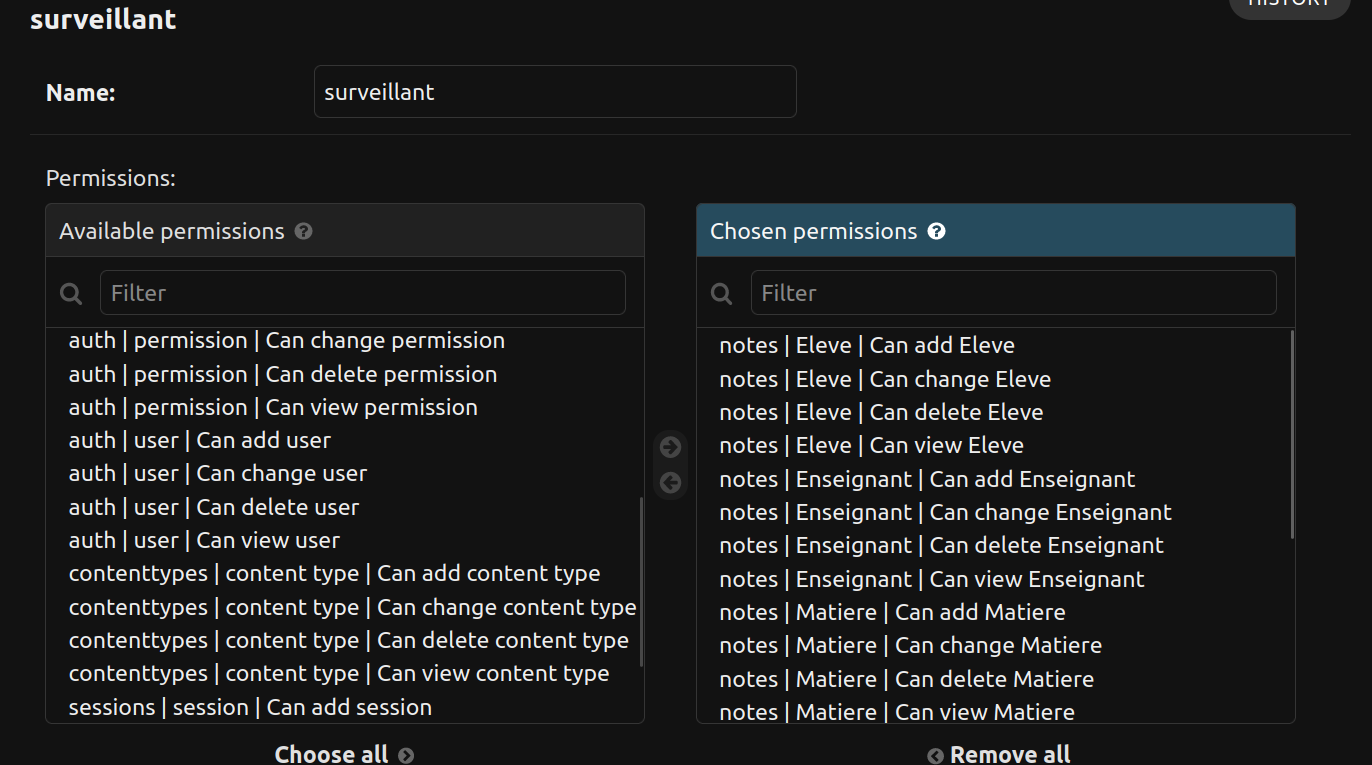
\includegraphics[scale=0.3]{images/3.png}
\end{center}
\item Django fournit une classe User qui contient l’ensemble des informations nécessaires à l’authentification
et aux autorisations Nous pouvons étendre ce modèle sans modifier nos modèles utilisateurs par défaut soit:
	\begin{itemize}
		\item En créant une relation d'héritage entre notre modèle et le modèle par défaut \textbf{Users}
		\item En créant une relation OneToOne entre notre modèle et le modèle par défaut \textbf{Users}
	\end{itemize}
\item Nous allons procéder à la création OneToOne entre les deux modèles, lorsqu'on lance \textbf{py manage.py makemigrations}, on a l'erreur suivante:
\begin{center}
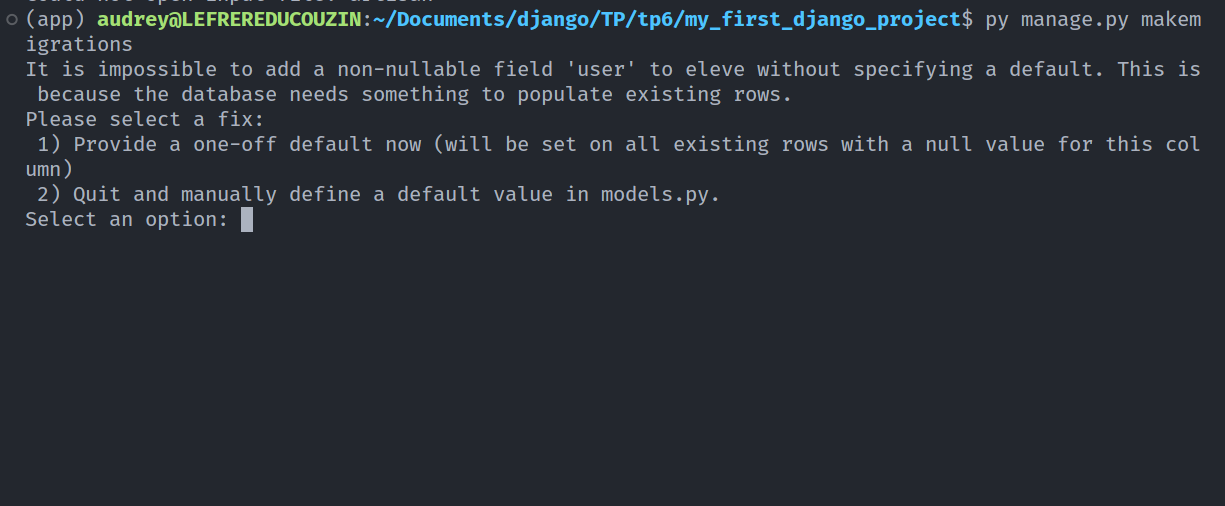
\includegraphics[scale=0.3]{images/error.png}
\end{center}
Ensuite on corrige le modèle en rendant l'attribut \textbf{user} nullable:
\begin{center}
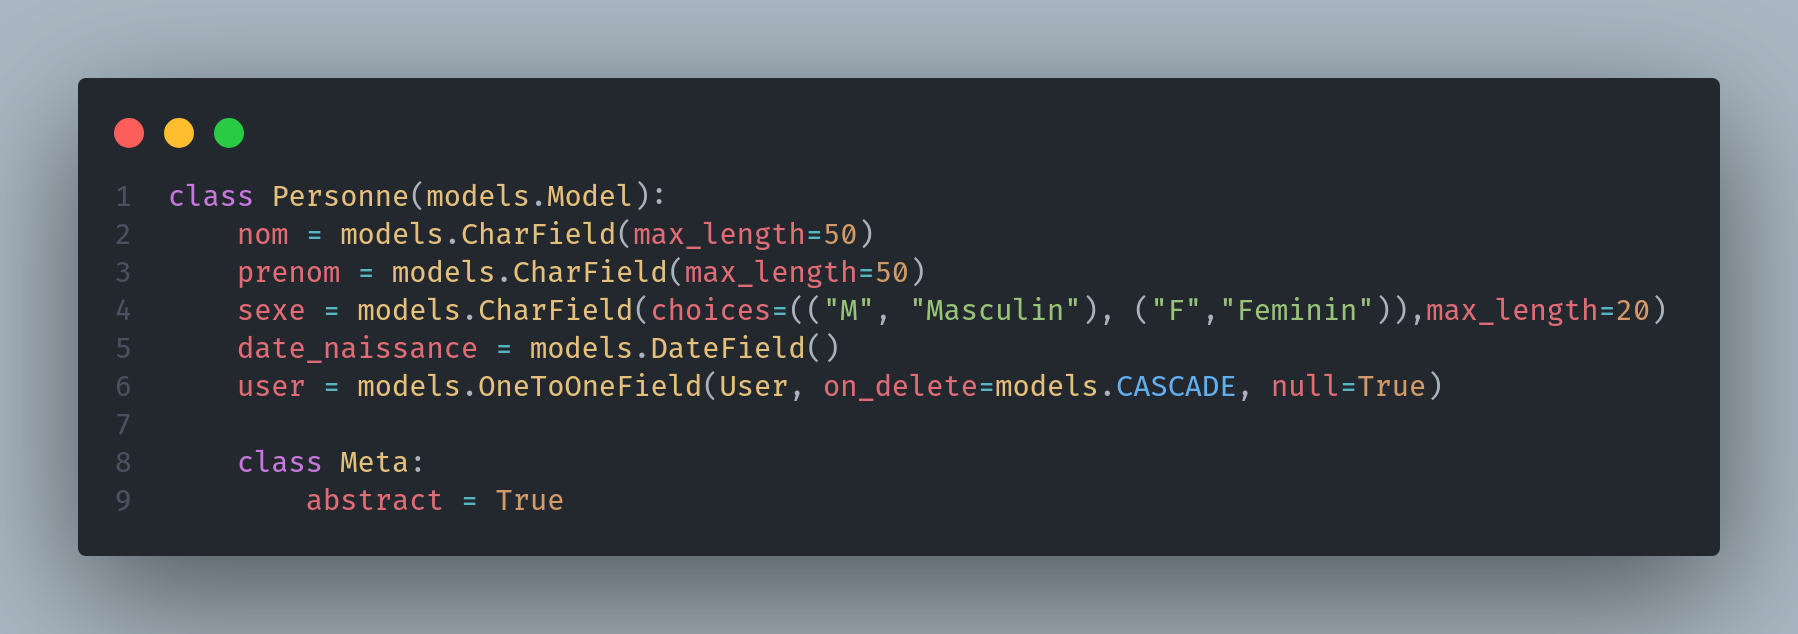
\includegraphics[scale=0.2]{images/per.png}
\end{center}
\item Nous allons maintenant créer une instance de \textbf{User} pour chaque personne que nous avions créé:

\begin{center}
	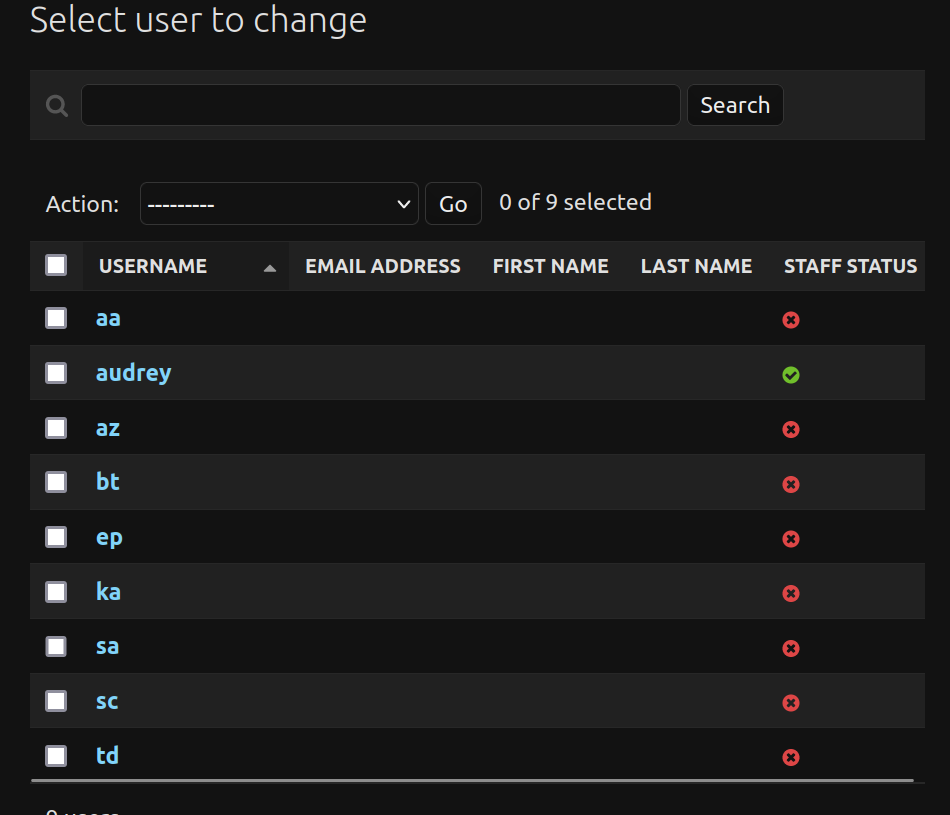
\includegraphics[scale=0.3]{images/users.png}
\end{center}
\item Nous allons maintenant enlever la propriété nullable sur l'attribut précédemment ajouter. Losqu'on essaie de relancer les migration, on a le message suivant au terminal:
\begin{center}
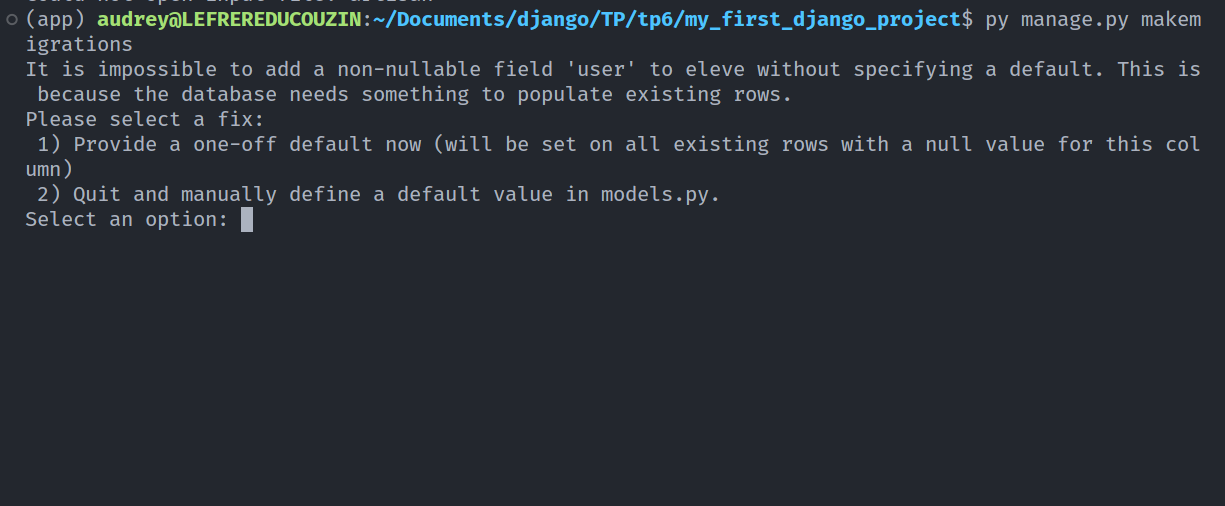
\includegraphics[scale=0.3]{images/error.png}
\end{center}
NOus allons ignorer en choississant k'option 3, puis nous allons aller dans le site administrateur et assigner les user aux différentes instances de personnes créées.
L'étape suivante ma consister à supprimer tout les fichiers présents dans le répertoire \textbf{/notes/migrations} sauf le fichier \textbf{\_\_init\_\_.py}
On relance la commande  \textbf{py manage.py makemigrations} et puis  \textbf{py manage.py migrate}. 
\item Pour l'instant dans mon application, il n'y a que la vue \textbf{add\_note} qui est restreinte à quelques utilisateurs. Nous allons donc faire en sorte qu'un utilisateur non authentifier et qui n'a pas les permissions requises ne puisse pas y accéder.
\begin{center}
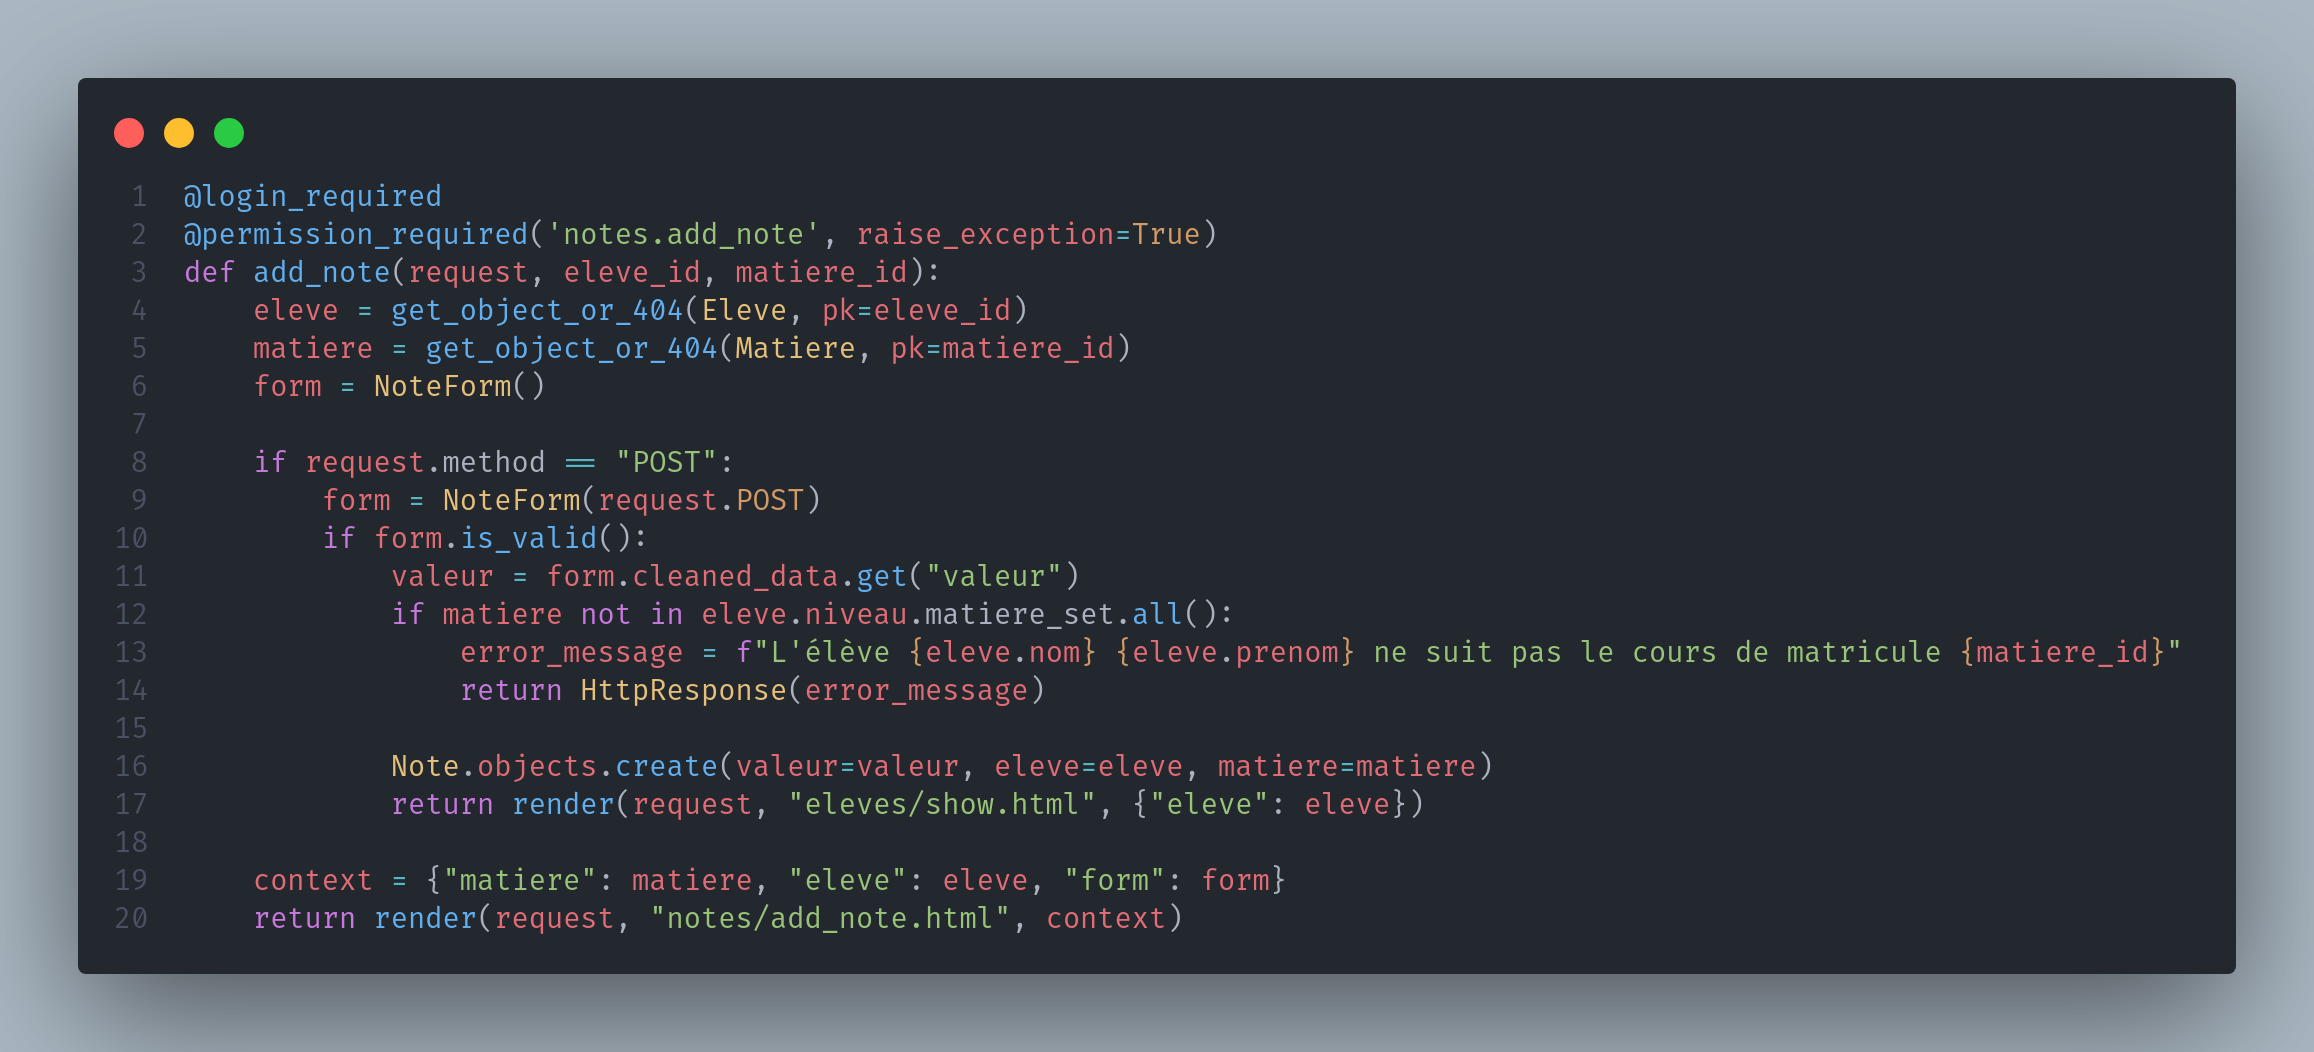
\includegraphics[scale=0.2]{images/cont.png}
\end{center}
Avant de tester cette fonctionnalité, nous allons mettre en place l'authentification des utilisateurs.
	\begin{itemize}
		\item \textbf{Ajout des urls d'auth} Dans le fichiers \textbf{/ifnti\_l3/urls.py}, nous allons ajouter les urls suivant \textbf{    path('accounts/', include('django.contrib.auth.urls')),} à l'urlspattern:
			\begin{center}
				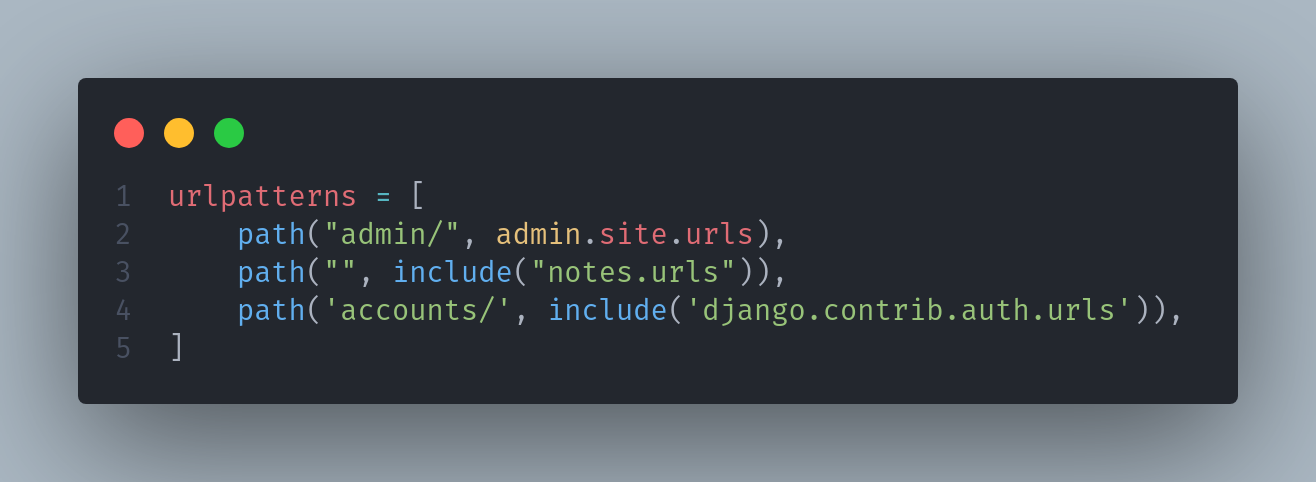
\includegraphics[scale=0.2]{images/authurl.png}
			\end{center}
			Lorsqu'on essaie d'accéder à l'urls /accounts, on a les erreurs suivantes:
	\begin{center}
				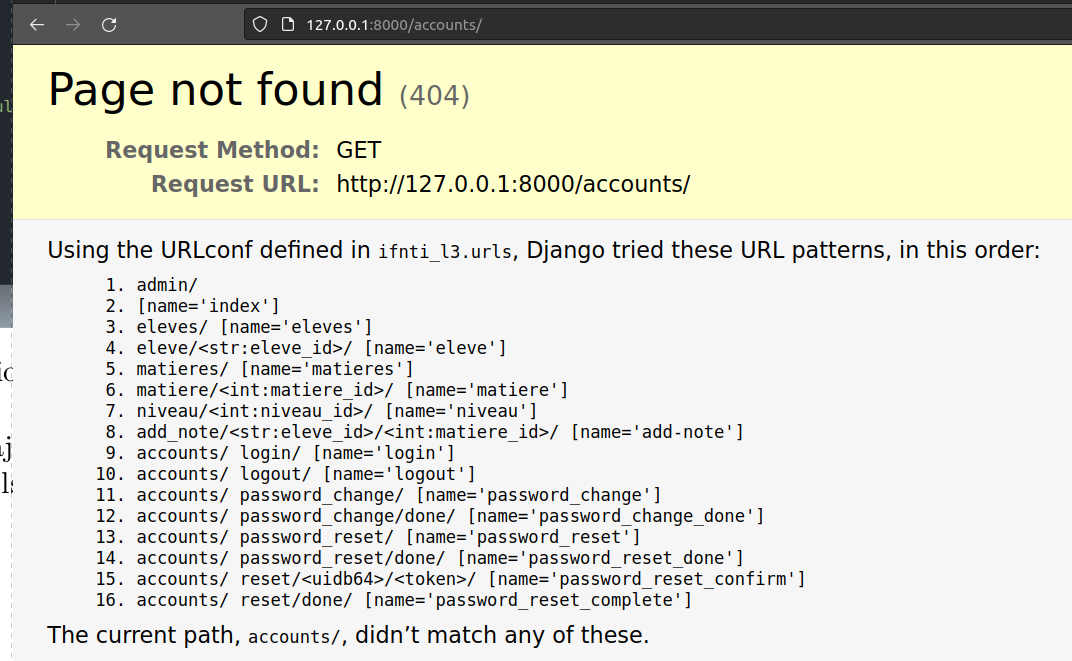
\includegraphics[scale=0.2]{images/autherr.png}
			\end{center}
			Django a parcouru tout les urls possible et n'a trouver aucune correspondance. Parmi la liste d'urls, on peut remarqué le /accounts/login. Essayons d'y accéder:
			\begin{center}
				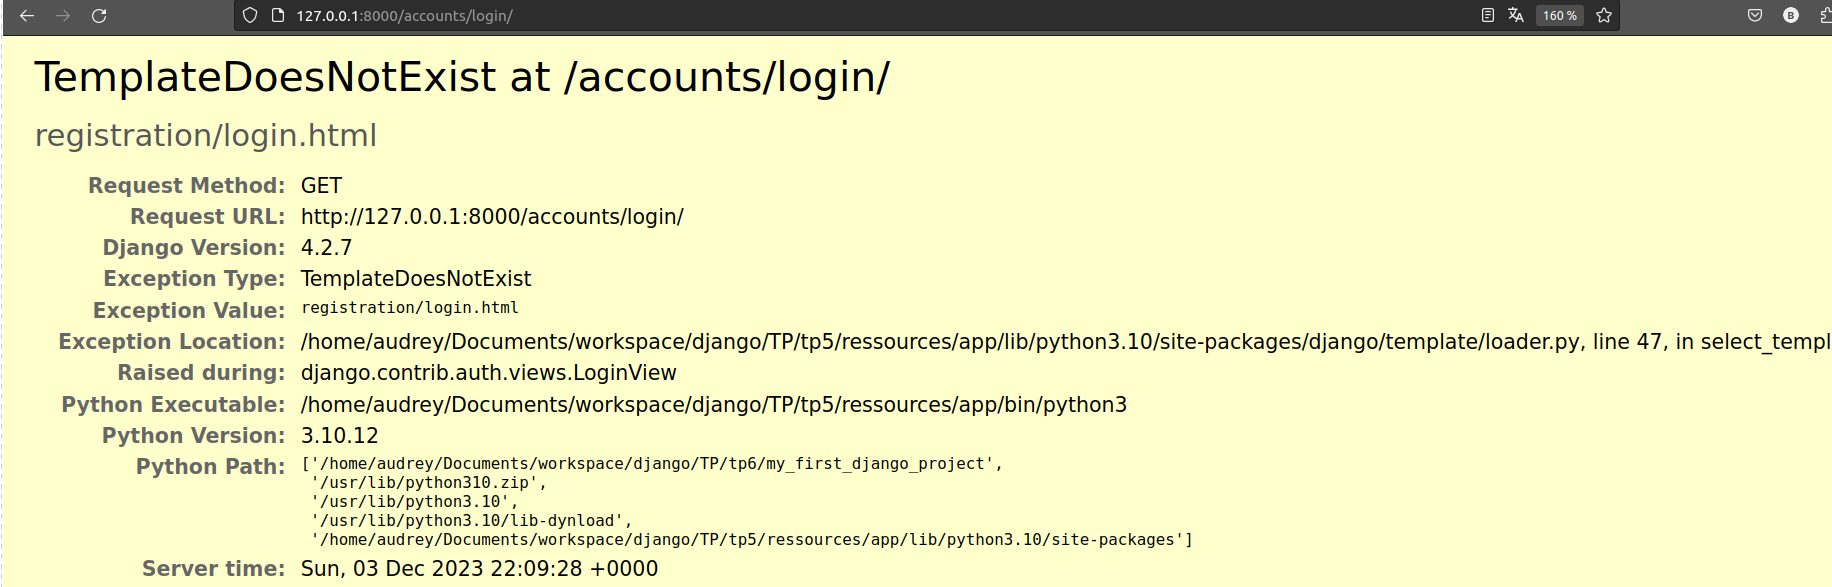
\includegraphics[scale=0.2]{images/autherrlog.png}
			\end{center}
			Cette erreur stipule que l'url existe mes il n'y a pas de template qui y ait associé. Et le template qui est recherché devrait etre registration/login 
		\item \textbf{Création des templates du template de connexion}
		Nos allons procéder à la création du template de connexion
		Tout d'abord, créons le répertoire \textbf{/templates/registration} à la racine du projet. Ensuite créons y le fichier \textbf{login.html}
		\begin{center}
				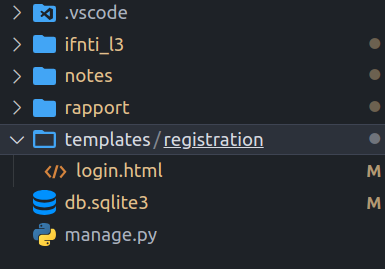
\includegraphics[scale=0.2]{images/arc.png}
								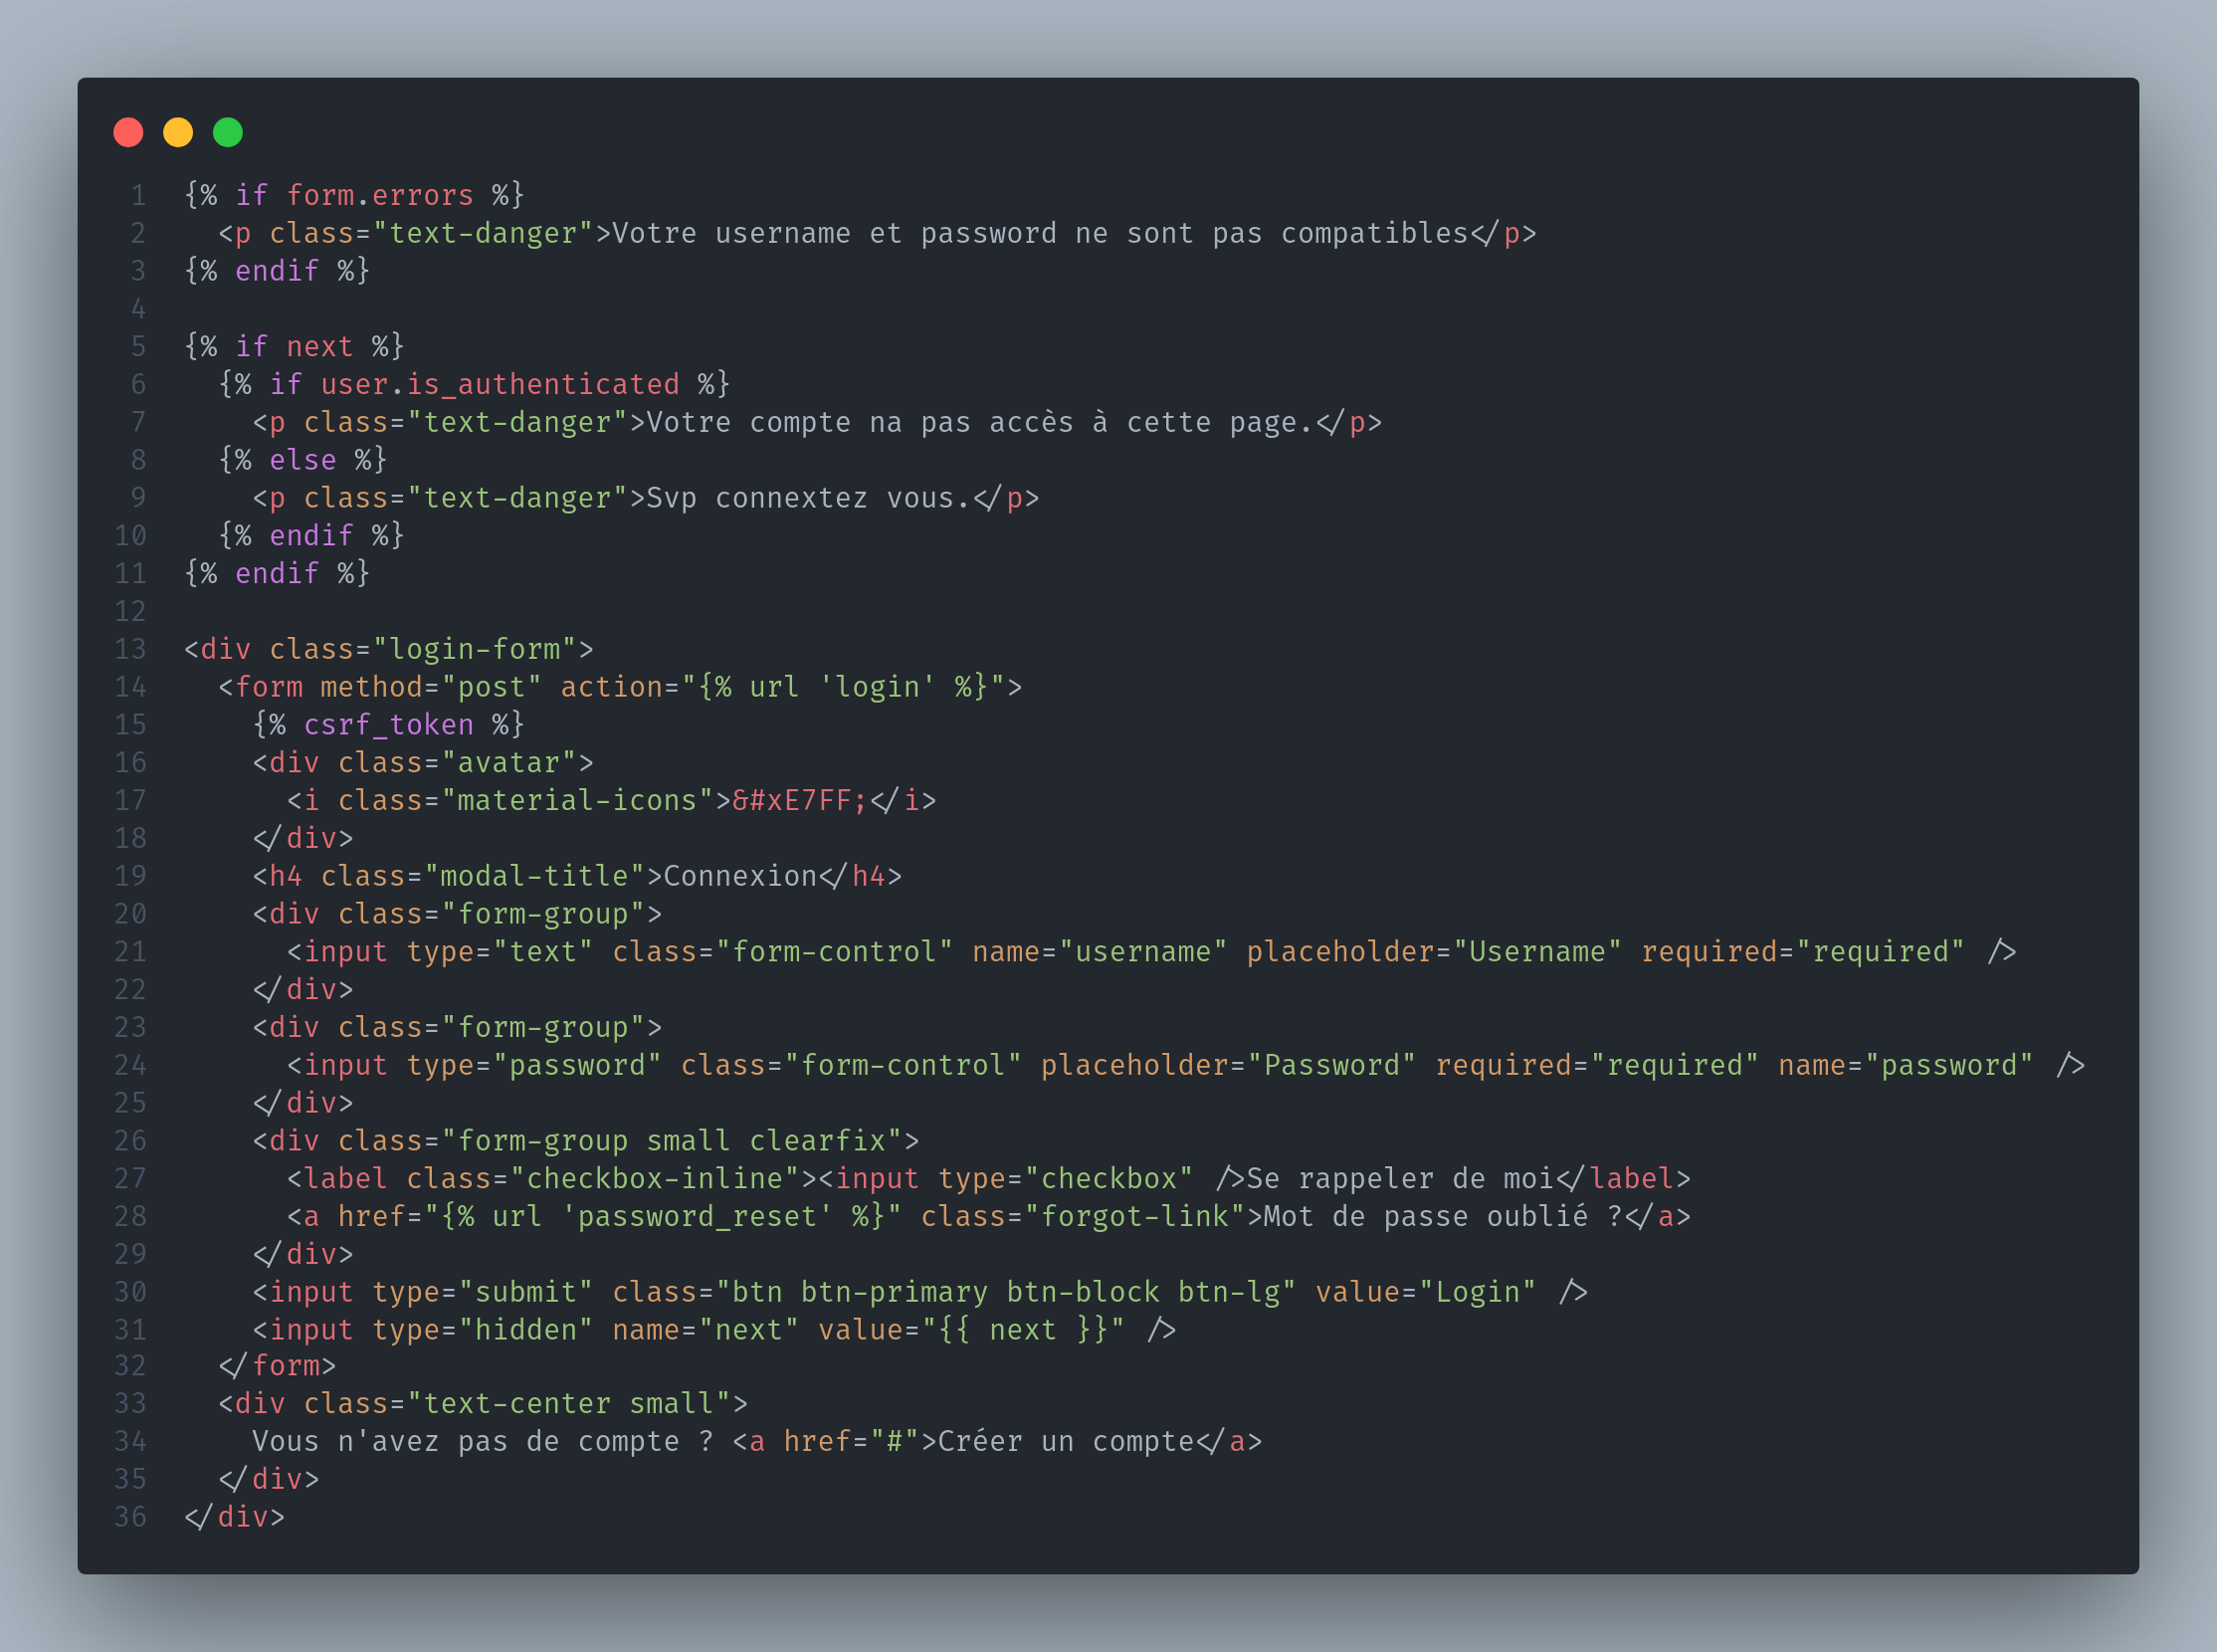
\includegraphics[scale=0.2]{images/login.png}
			\end{center}
				Puis dans le fichier de configuration du projet \textbf{/ifnti\_l3/settings.py} nous allons rende le répertoire template accessible. Apès modification, la liste TAMPLATE devrait ressembler à ceci( ne pas oublier d'importer os):
	\begin{center}
				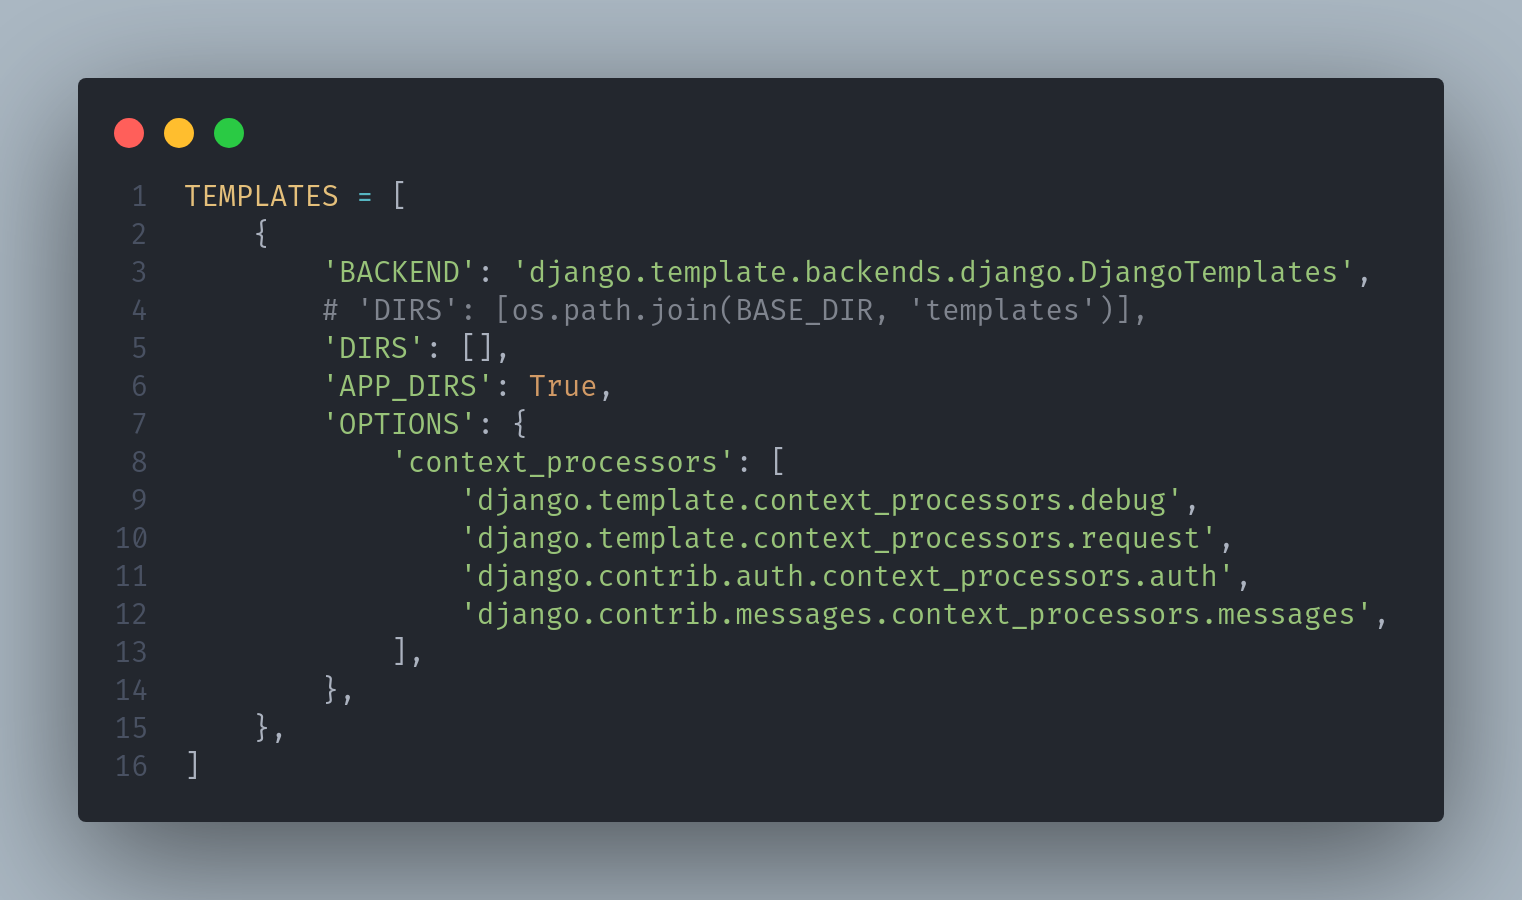
\includegraphics[scale=0.2]{images/templ.png}
								
			\end{center}
			Par défaut, apres la connexion, django redirige vers l'url \textbf{/accounts/profile}. Nous allons changer cela
	\item \textbf{Redirection} Dans le même fichier spécifier l'url de redirection apres la connexion: on ajoute ceci au ficher: \textbf{
LOGIN\_REDIRECT\_URL = '/'}
Maintenant les utilisateurs peuvent s'authentifier.
	\end{itemize}

	\item A présent, nous somme capable de tester les contraintes ajouter à la vue. 
	Je me suis authentifier en tant qu'eleve et voici le resultat quand je tente d'acceder à la vue:
		\begin{center}
				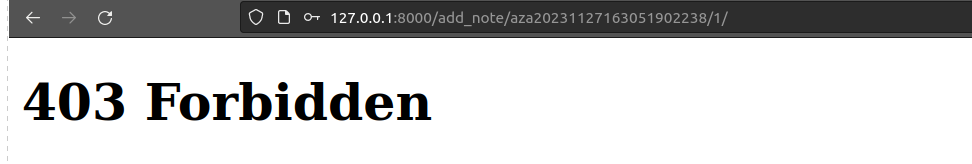
\includegraphics[scale=0.2]{images/403.png}
								
			\end{center}
			avec un compte enseignant, aucune erreur ne survient.
\end{enumerate}
\section{Les problèmes de sécurité}
\begin{enumerate}
	\item Les attaques XSS permettent à un intrus d’injecter des scripts clients dans les navigateurs des utilisateurs. Le principe général est de stocker les scripts malveillants dans la base de données d’où ils seront repris et affichés pour d’autres utilisateurs, ou encore d’amener les utilisateurs à cliquer sur un lien qui va provoquer l’exécution du JavaScript de l’attaquant dans le navigateur des utilisateurs. Cependant, les attaques XSS peuvent provenir de n’importe quelle source de données non fiable, comme les cookies ou les services Web, à chaque fois que les données ne sont pas suffisamment nettoyées avant d’être incluses dans une page.
	Les gabarits de Django échappent des caractères spécifiques qui sont particulièrement dangereux en HTML. Bien que cela protège les utilisateurs de la plupart des saisies malveillantes, cela ne constitue pas une protection absolue. 
	\item Les attaques CSRF permettent à une personne malveillante d’exécuter des actions en utilisant les données d’authentification d’un autre utilisateur sans que ce dernier ne s’en rende compte.
	Django offre une protection intégrée contre la plupart des types d’attaques CSRF, pour autant que vous l’ayez activée et que vous l’utilisiez de manière appropriée. Toutefois, comme pour toute technique de protection, elle est limitée. Par exemple, il est possible de désactiver le module CSRF de manière globale ou pour certaines vues. Vous ne devriez le faire que si vous savez ce que vous faites. Il existe d’autres limites si votre site contient des sous-domaines qui ne sont pas sous votre contrôle.
	\item L’injection SQL est un type d’attaque où un utilisateur malveillant est capable d’exécuter du code SQL arbitraire sur une base de données. Il peut en résulter des suppressions d’enregistrements ou des divulgations de données.
	Les jeux de requête de Django sont prémunies contre les injections SQL car leurs requêtes sont construites à l’aide de la paramétrisation des requêtes. Le code SQL d’une requête est défini séparément de ses paramètres. Comme ceux-ci peuvent provenir de l’utilisateur et donc non sécurisés, leur échappement est assuré par le pilote de base de données sous-jacent.
	\item Le détournement de clic est un type d’attaque où un site malveillant intègre un autre site dans un cadre. Cette attaque peut amener un utilisateur à cliquer de manière non désirée pour effectuer des actions non volontaires sur le site ciblé.Django intègre une protection contre le détournement de clic sous la forme de l'intergiciel X-Frame-Options qui, dans un navigateur qui le prend en charge, peut empêcher un site d’être affiché à l’intérieur d’un cadre. Il est possible de désactiver cette protection par vue ou de configurer la valeur exacte de l’en-tête envoyé.
	\item Le déploiement de votre site en HTTPS est toujours mieux pour la sécurité. Sans cela, il est possible que des utilisateurs malveillants du réseau interceptent des données d’authentification ou toute autre information transférée entre le client et le serveur et, dans certains cas, pour des attaquants réseau actifs, que des données soient modifiées au passage, dans l’une ou l’autre direction.
Si vous souhaitez profiter de la protection ajoutée par HTTPS et l’activer sur votre serveur, il peut être nécessaire de procéder à quelques étapes supplémentaires :
    Utilisez Sécurité de transport HTTP stricte (HSTS)
    HSTS est un en-tête HTTP informant le navigateur que toute connexion future à un site particulier devra toujours utiliser HTTPS. Combiné avec la redirection des requêtes HTTP vers HTTPS, cela garantit que les connexions profiteront toujours de la sécurité ajoutée par SSL à partir du moment où une connexion réussie a eu lieu. 
    \item Django utilise l’en-tête Host fourni par le client pour construire les URL dans certains cas. Même si ces valeurs sont vérifiées pour empêcher les attaques Cross Site Scripting, une valeur Host contrefaite peut être exploitée pour des attaques de type Cross-Site Request Forgery, d’empoisonnement de cache et d’empoisonnement de liens dans les courriels.Comme même des configurations de serveur Web apparemment sûres sont susceptibles d’accepter des en-têtes Host contrefaits, Django valide les en-têtes Host en les comparant avec le réglage ALLOWED\_HOSTS dans la méthode django.http.HttpRequest.get\_host().\\
    Il n’existe actuellement pas de solution technique à toute épreuve dans l’infrastructure Django pour valider de manière sûre tous les contenus de fichiers envoyés par les utilisateurs. Cependant, il existe un certain nombre de mesures à prendre pour diminuer les risques de telles attaques :
    \begin{itemize}
    	\item Une catégorie d’attaques peut être évitée en servant toujours les contenus envoyés par les utilisateurs à partir d’un autre nom de domaine de premier ou de deuxième niveau.
    	\item En plus de cette mesure, les applications peuvent choisir de définir une liste des extensions de fichiers autorisées pour les fichiers téléversés par les utilisateurs et configurer le serveur Web pour qu’il n’accepte de servir que ces fichiers.
    \end{itemize}
    Les sous-domaines d’un site peuvent définir des cookies pour le client valables pour tout le domaine. Cela rend possible les attaques par fixation de session si des cookies peuvent être créés par des sous-domaines qui ne sont pas sous contrôle de personnes de confiance.

Par exemple, un attaquant pourrait se connecter à good.example.com et obtenir une session valable pour son compte. Si l’attaquant contrôle bad.example.com, il peut l’utiliser pour vous envoyer sa clé de session puisqu’un sous-domaine a le droit de définir des cookies pour *.example.com. Lorsque vous visitez good.example.com, vous serez connecté sous le compte de l’attaquant et vous pourriez saisir involontairement des données personnelles sensibles (par ex. des données de carte de crédit) enregistrées dans le compte de l’attaquant.

Une autre attaque possible apparaît dans le cas où good.example.com définit son réglage SESSION\_COOKIE\_DOMAIN à "example.com", ce qui pourrait avoir comme conséquence d’envoyer les cookies de session à bad.example.com.
\end{enumerate}
\section{Customiser le site d'administration}
\begin{enumerate}
	\item Il est interressant de modifier le site admin pour les ajouter certaines fonctionnalités, qui n'existe pas par défaut.
	\item Il est possible d'utiliser les ModelAdmin pour rendre les modèles accessibles dans le site admin
	\item Explication des options 
		\begin{itemize}
		\item Attribuez à \textbf{date\_hierarchy} le nom d’un champ DateField ou DateTimeField de votre modèle, et la page de liste pour modification inclura une navigation par filtres sélectifs basés sur les dates en fonction de ce champ.
		\item Définissez \textbf{list\_filter} pour activer des filtres dans la barre de droite de la page de liste pour modification de l’administration.
		\item Définissez \textbf{list\_display} pour contrôler quels champs sont affichés sur la page de liste pour modification de l’interface d’administration.
		\item Utilisez \textbf{list\_display\_links} pour contrôler le cas échéant quels champs de \textbf{list\_display} doivent faire le lien vers la page de modification d’un objet.
		\item Définissez \textbf{list\_editable} à une liste de noms de champs de modèle afin de permettre l’édition de ces champs sur la page de liste pour modification. C’est-à-dire que les champs répertoriés dans \textbf{list\_editable} seront affichés sous forme de composants de formulaire sur la page de liste pour modification, permettant aux utilisateurs de modifier et d’enregistrer plusieurs lignes à la fois.
		\item Utilisez l’option \textbf{fields} si vous avez besoin de réaliser de simples changements dans la disposition des formulaires des pages « ajouter » et « modifier », comme afficher uniquement un sous-ensemble des champs disponibles, modifier leur ordre ou les regrouper en lignes.
		\item Cet attribut, si fourni, doit être une liste de noms de champs à exclure du formulaire.
		\item \textbf{raw\_id\_fields} est une liste de champs que vous souhaitez modifier par un simple composant Input, que ce soit un champ ForeignKey ou ManyToManyField.
		\item Définissez \textbf{show\_full\_result\_count} pour définir si le nombre total d’objets doit être affiché sur une page d’administration filtrée (par exemple 99 résultats (103 au total)). Si cette option est définie à False, un texte du style 99 résultats (tout afficher) s’affiche à la place.
		\item Si vous souhaitez désactiver le tri pour certaines colonnes, définissez \textbf{sortable\_by} à une collection (par ex. list, tuple ou set) sous-ensemble de \textbf{list\_display} qui sont susceptibles d’être triés. Une collection vide désactive le tri pour toutes les colonnes.
		\item Par défaut, un champ ManyToManyField est affiché dans le site d’administration avec un <select multiple>. Cependant, les boîtes à sélection multiple peuvent être difficiles à utiliser lors de la sélection de nombreux éléments. En ajoutant un champ ManyToManyField à cette liste, cette boîte sera remplacée par une discrète et astucieuse interface de « filtre » JavaScript permettant de rechercher dans les options. Les options non sélectionnés et sélectionnés apparaissent dans deux boîtes côte à côte. Voir \textbf{filter\_vertical} pour utiliser une interface verticale.
		\item  \textbf{filter\_vertical}   Identique à \textbf{filter\_horizontal}, mais utilise un affichage vertical de l’interface de filtre avec la boîte d’options non sélectionnées apparaissant au-dessus de la boîte d’options sélectionnées.
		\item     La chaîne à utiliser pour l’affichage de valeurs vides dans la liste pour modification du site d’administration. Il s’agit par défaut d’un tiret. La valeur peut aussi être surchargée sur la base des classes ModelAdmin ou sur un champ précis d’une classe ModelAdmin en définissant un attribut \textbf{empty\_value\_display} pour le champ. Voir \textbf{ModelAdmin.empty\_value\_display} pour des exemples.
		\item     Définissez \textbf{list\_per\_page} pour contrôler le nombre d’éléments paginés apparaissant sur chaque page de la liste pour modification de l’administration. Par défaut, cette option est définie à 100.
		\item Définissez \textbf{save\_as} pour activer la fonctionnalité « enregistrer comme nouveau » des formulaires d’édition de l’administration.
		\item     Lorsque \textbf{save\_as}=True, la redirection par défaut après l’enregistrement du nouvel objet se fait vers la vue pour modification de cet objet. Si vous définissez \textbf{save\_as\_continue}=False, la redirection se fera vers la vue de liste pour modification.

    Par défaut, \textbf{save\_as\_continue} est défini à True.
		\item Si \textbf{readonly\_fields} est utilisé sans ordre explicite défini par \textbf{ModelAdmin.fields} ou \textbf{ModelAdmin.fieldsets}, ils seront ajoutés en dernier après tous les champs modifiables.

Un champ en lecture seule n’est pas limité à l’affichage des données d’un champ de modèle, il peut également afficher le résultat d’une méthode de modèle ou d’une méthode de la classe \textbf{ModelAdmin}. C’est très similaire à la façon dont \textbf{ModelAdmin.list\_display} fonctionne. Cela fournit un moyen pour faire présenter à l’interface d’administration des informations sur l’état des objets en cours d’édition.
		\item     Définissez \textbf{save\_on\_top} pour ajouter les boutons d’enregistrement au sommet des formulaires d’édition de l’administration.

    Normalement, les boutons d’enregistrement apparaissent uniquement au bas des formulaires. Si vous définissez \textbf{save\_on\_top}, les boutons apparaîtront à la fois en haut et en bas.

    Par défaut, \textbf{save\_on\_top} est défini à False.
		\item Définissez \textbf{search\_fields} pour activer une boîte de recherche sur la page de liste pour édition de l’administration. Cet attribut doit contenir une liste de noms de champs qui seront recherchés chaque fois que quelqu’un soumet une requête de recherche dans cette zone de texte.
		\item Définissez \textbf{view\_on\_site} pour contrôler l’affichage du lien « Voir sur le site ». Ce lien est censé diriger vers une URL où l’objet enregistré peut être affiché.
		\end{itemize}
	\item NOus allons tester une option, readonly\_fields.
		\begin{center}
			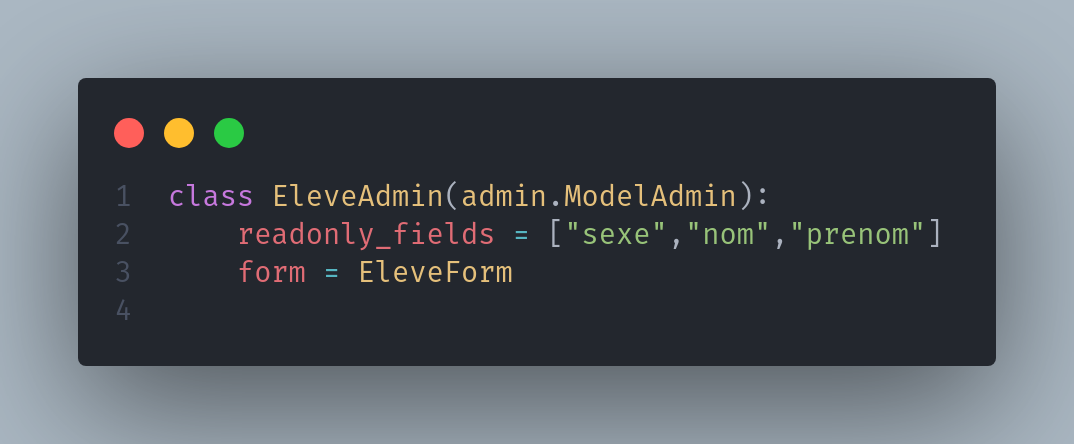
\includegraphics[scale=0.2]{images/reado.png}
						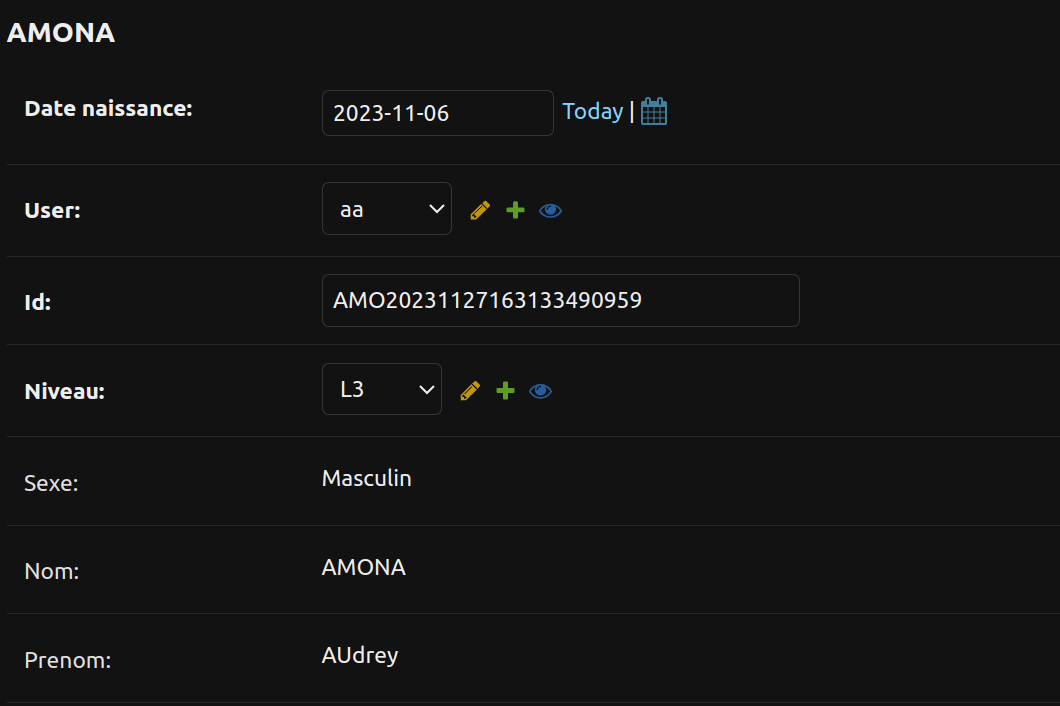
\includegraphics[scale=0.2]{images/read.png}
		\end{center}
		On remarque que le nom, le prenom et le sexe de l'eleve ne sont plus modifiable
		\item Il est possible de modifier les templates par défaut du site adonistrateur, en créant un dossier \textbf{admin} dans un répertoire \textbf{template} qui est enregistré dans le settings.py. Ensuit il faudra copier les templates que l'on souhaite modifier depuis le répertoire \textbf{/django/contrib/admin/templates/admin} vers le répertoire créé. Il est possible de modifier les templates admin juste pour un modèles donné, dans ce cas il faudra ajouter dans le répertoire admin créé un répertoire portant le nom du mod-le mais tout en minuscule. ensuite la copie est faite vers ce répertoire. 
		\item Il est possible d'inclure des fichiers js et css personnalisé en les ajoutant dans le répertoire \textbf{/django/contrib/admin/static/admin/css|js} et en les ajoutant au html par le base.html des templates admins
		\item Par défaut, l'entête des pages du site d'administration de Django est généré par le fichier de template admin/base\_site.html. Ce template définit la structure de base de l'interface d'administration, y compris l'entête.
\end{enumerate}
\end{document}